\hypertarget{Design}{\chapter{Design}}

\section{Motivace}

Při tvorbě aplikace bylo neustále nutné myslet na dva hlavní faktory, kolem kterých se celý design musí odvíjet; to sice, že je program mířený pro dvě skupiny: učitele a žáky zároveň. 

Úkolem žáka je v časovém limitu odpovědět na jazykové otázky. Žák by měl mít co nejméně možností, jak podvádět, aby byl správně umístěn do jazykové skupiny úměrné jeho znalostem; dostane náhodnou sadu otázek různých obtížností, které pro jeho ročník navolí učitel.

Učitel pracuje se svým vlastním rozhraním, kde zadává otázky, vytváří testy, kontroluje průběh testování a získává automaticky zpracované výsledky.

V obou případech je důležité, aby byla webová aplikace intuitivní na používání, měla příjemný design a hlavně spolehlivě fungovala.

\section{Přihlašování}
\label{sec:login-design}

Ještě před tím, než se uživatelé dostanou do svého rozhraní, je potřeba, aby se přihlásili. Tato část aplikace je společná pro žáky i učitele. 

\begin{figure}[H]
    \centering
    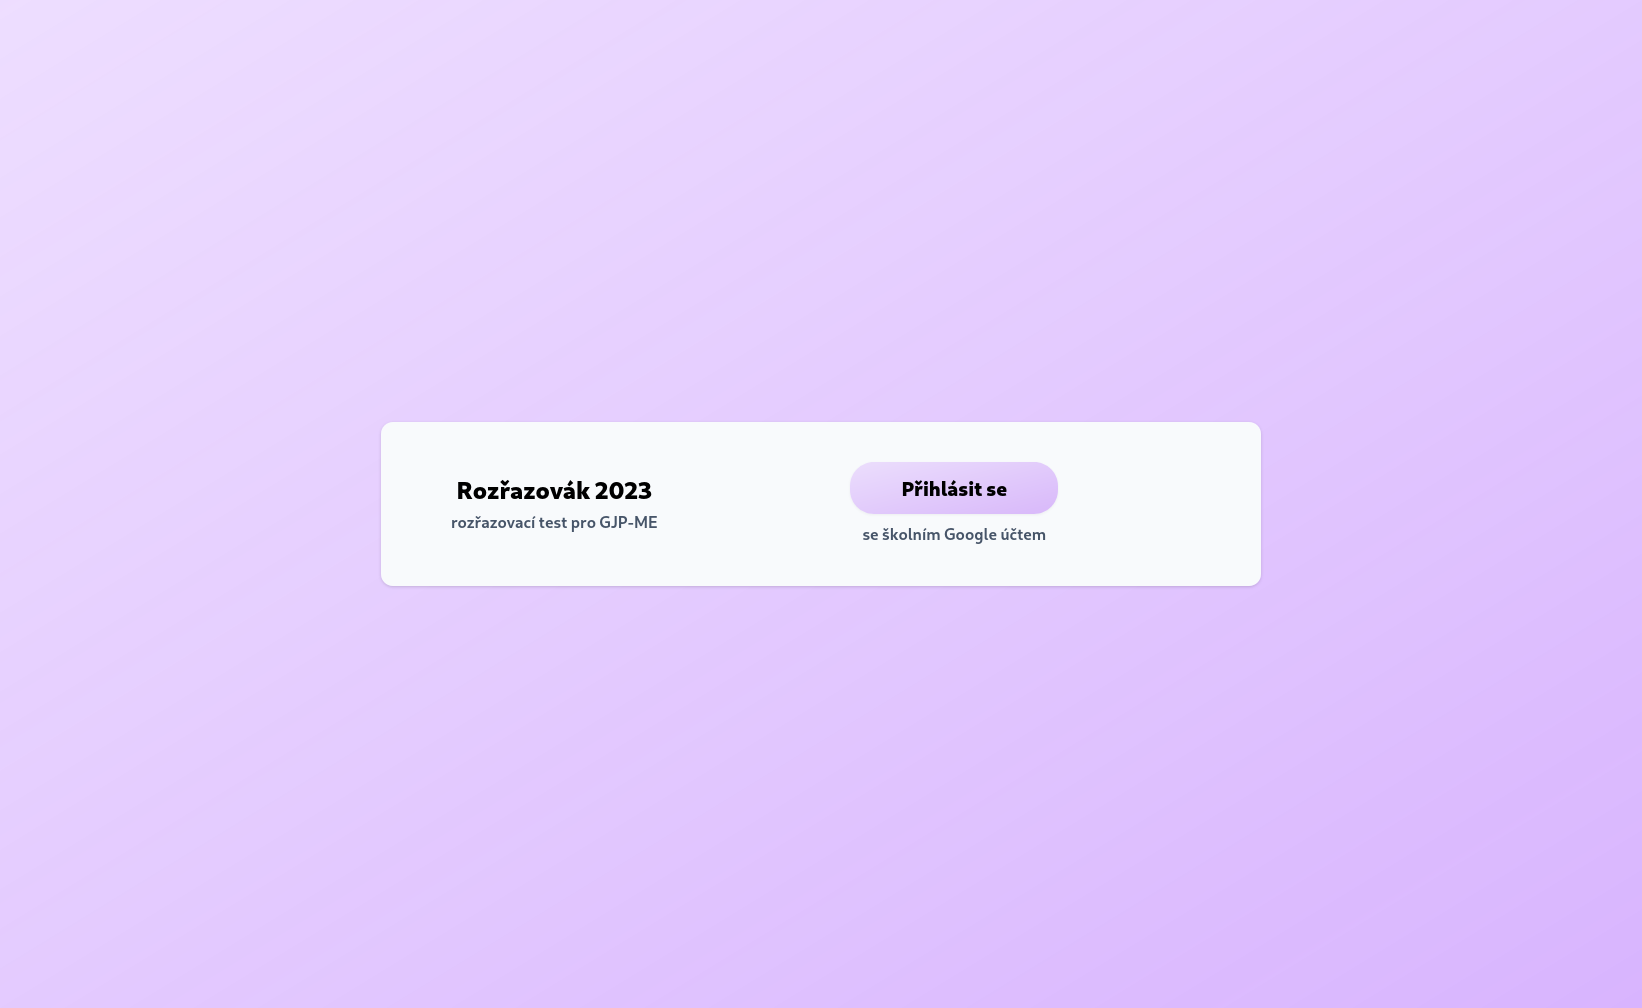
\includegraphics[width=350px]{images/01design/login.png}
    \caption{Přihlašovací stránka je hlavní stránkou aplikace.}
\end{figure}

Učitelé a žáci se přihlásí pomocí svého školního Google účtu (vizte \ref{sec:login}).

\newpage

Pokud se přihlásí učitel, zobrazí se nabídka pro přechod do administrátorské sekce.

\begin{figure}[H]
    \centering
    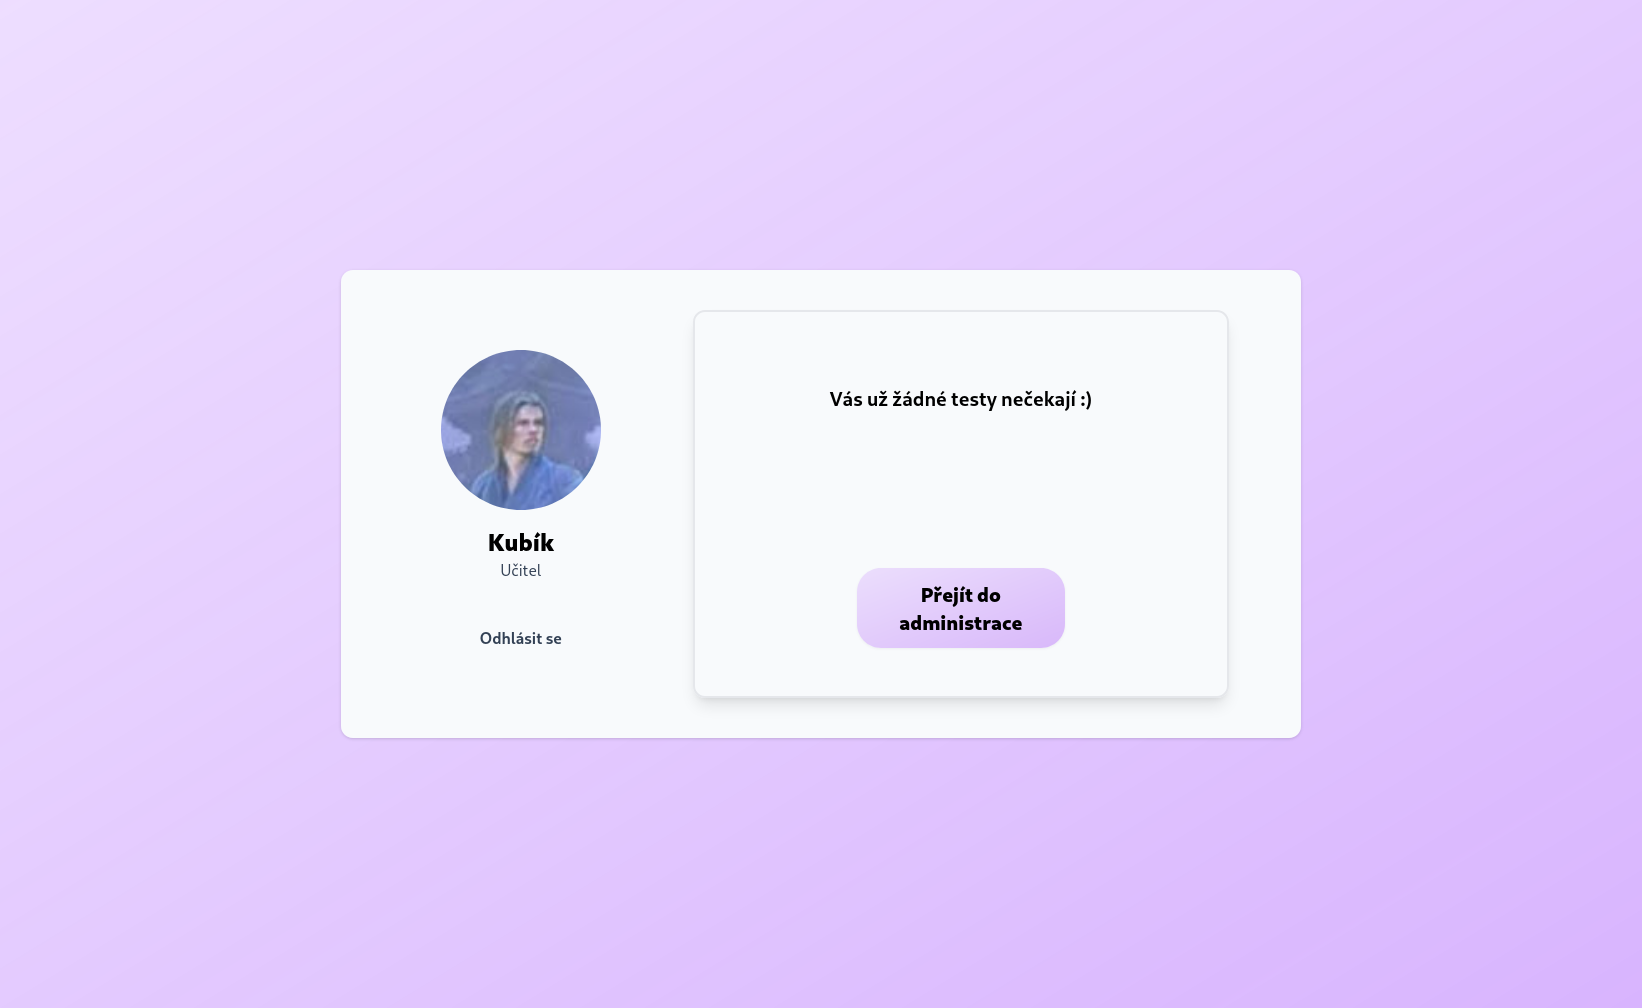
\includegraphics[width=350px]{images/01design/teacher.png}
    \caption{Hlavní stránka po přihlášení učitele.}
\end{figure}

Pokud se přihlásí žák, ve výchozím stavu se mu zobrazí stránka s informací, že pro něj aktuálně není spuštěný žádný test.

\begin{figure}[H]
    \centering
    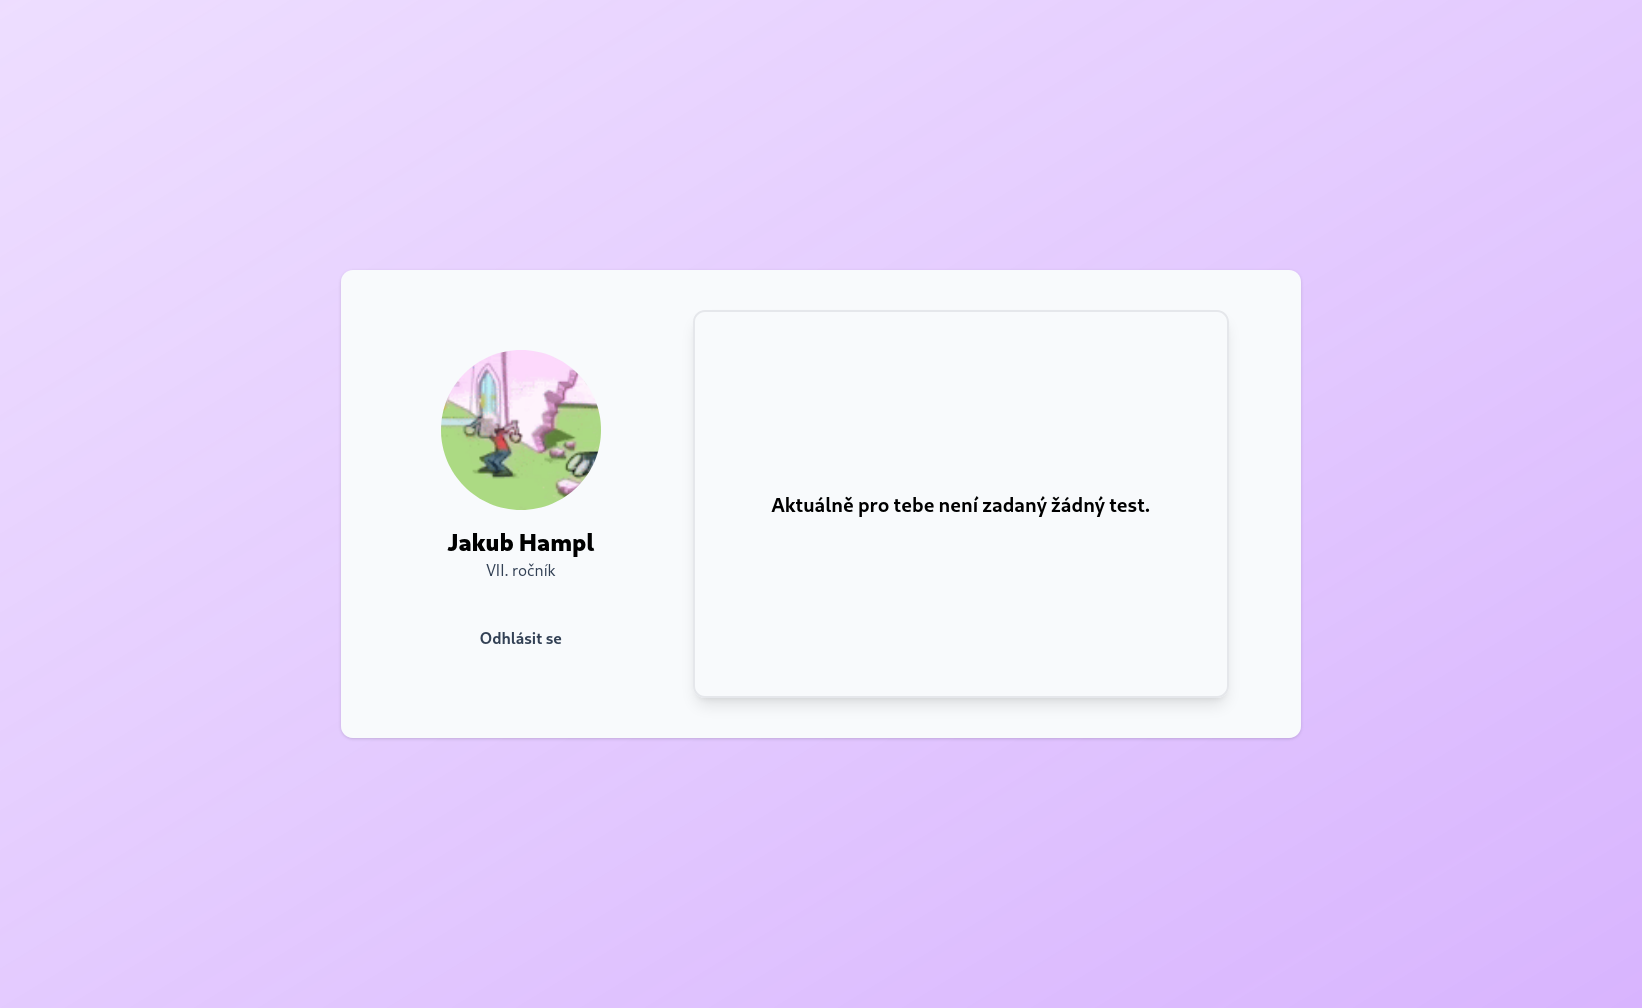
\includegraphics[width=350px]{images/01design/student-no-test.png}
    \caption{Hlavní stránka po přihlášení žáka bez zadaného testu.}
\end{figure}

Pokud je pro ročník přihlášeného žáka aktuálně aktivovaný test, je vidět jeho délka, počet otázek a obtížnost. Pokud ne, zobrazí se pouze informace o tom, že pro žáka žádný test aktuálně spuštěný není.

\begin{figure}[H]
    \centering
    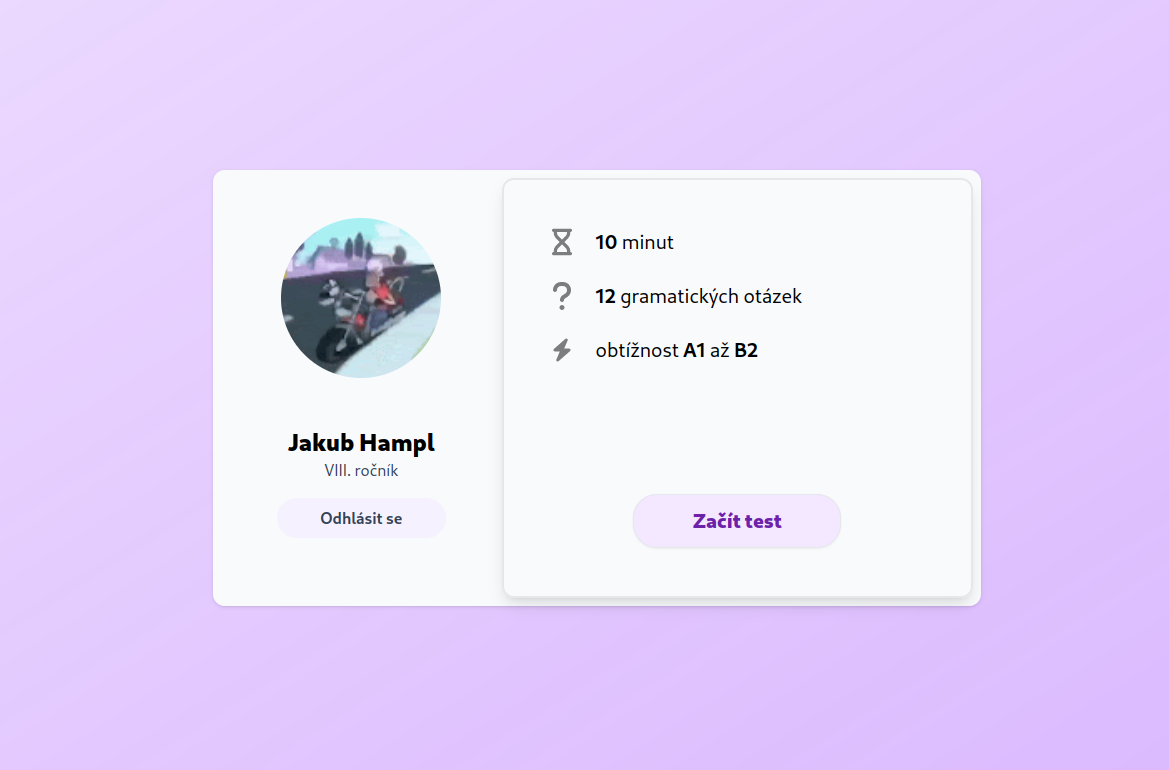
\includegraphics[width=350px]{images/01design/student-yes-test.png}
    \caption{Hlavní stránka po přihlášení žáka se zadaným testu.}
\end{figure}

Při aktivovaném testu může žák test spustit. Po spuštění se pro žáka vygeneruje originální sada otázek (vizte ODKAZ) a žák je přesměrován do žákovského rozhraní. Pokud žák během testu tuto stránku opustí (například kvůli technickým potížím, výpadku proudu, atp.), zůstává test spuštěný a je možné pokračovat v jeho vyplňování z hlavní stránky. 

\begin{figure}[H]
    \centering
    
\includegraphics[width=200px]{images/01design/continue.png}
    \caption{Při probíhajícím testu se text tlačítka změní na "Pokračovat" a zobrazí se pod ním zbývající čas.}
\end{figure}

Jakmile žák test odevzdá, je přesměrován zpět na hlavní stránku, kde mu je sdělen jeho výsledek.

\begin{figure}[H]
    \centering
    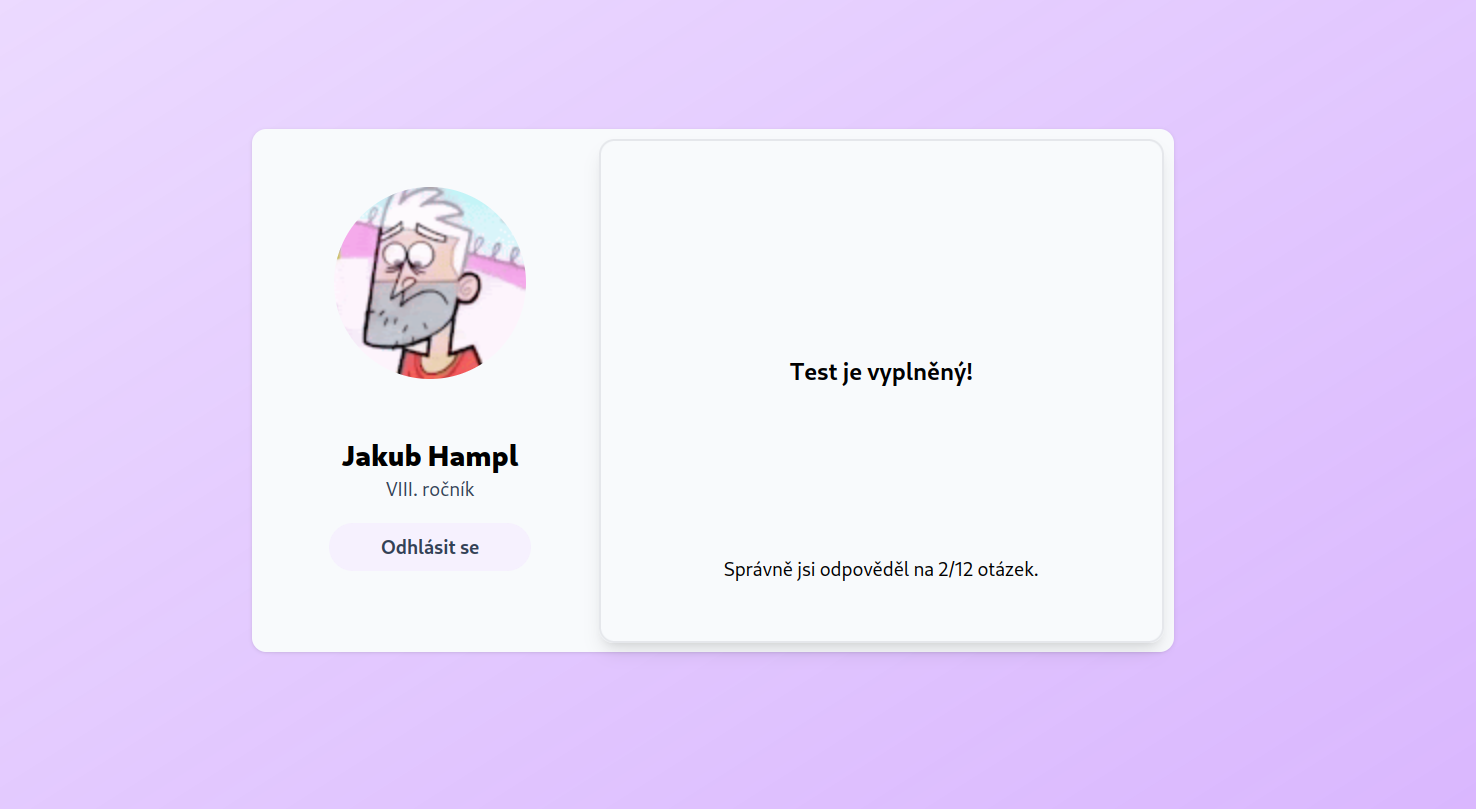
\includegraphics[width=350px]{images/01design/filled-out.png}
    \caption{Hlavní stránka s výsledky po odevzdání testu.}
\end{figure}

V případě, že žák na testování chyběl a stránku si zobrazí poté, co je test učitelem ukončen, zobrazí se mu tato informační stránka.

\begin{figure}[H]
    \centering
    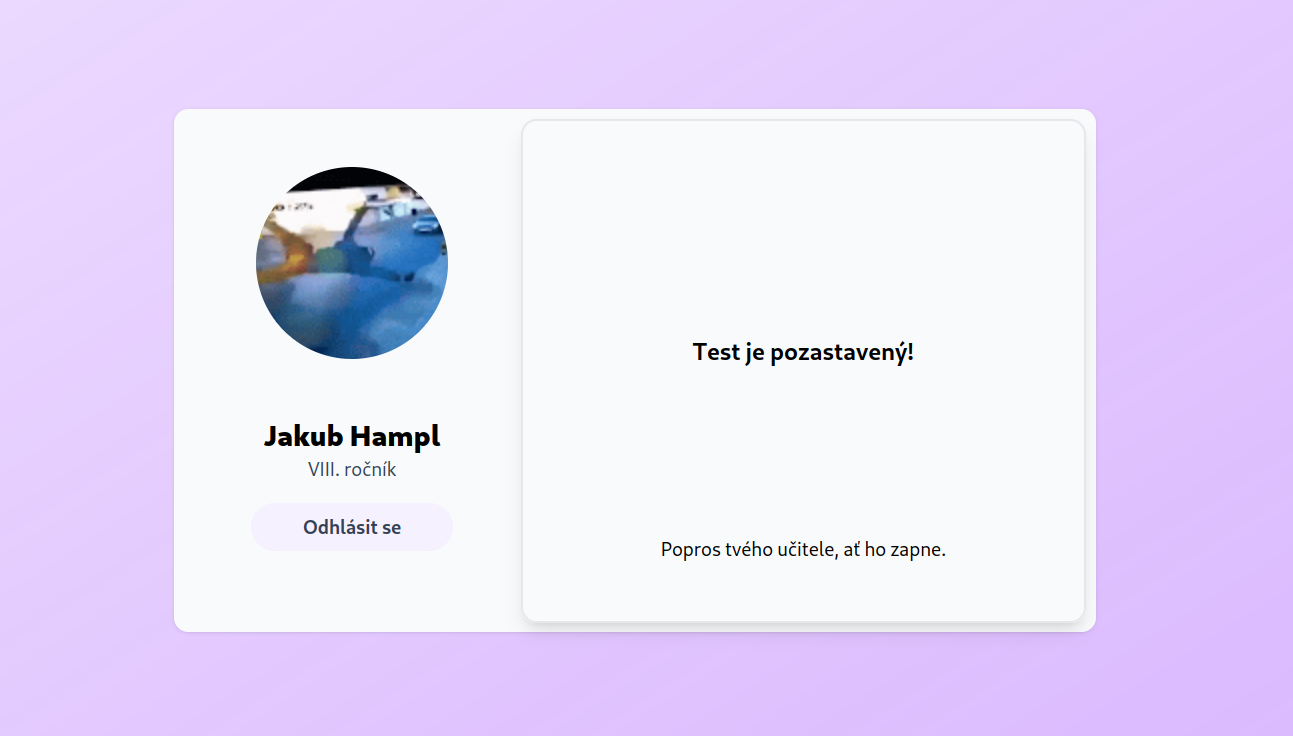
\includegraphics[width=350px]{images/01design/pending.png}
    \caption{Hlavní stránka s informací o pozastavení testu.}
\end{figure}

\section{Žákovské rozhraní}

Žákovské rozhraní slouží k vyplňování vygenerovaných testů. Pro každý ročník je předem nastavený čas a počet otázek různých obtížností (vizte xxx). Z banky otázek je podle těchto kritérií několik náhodně vybráno a zobrazeno. Otázky mohou být růyného druhu, ale u každé otázky je vždy na výběr ze čtyř možností z nichž právě jedna je správná. 

\section{Učitelské rozhraní}
\label{sec:admin}
